\documentclass{article}

\usepackage{graphicx}
\usepackage{physics}
\usepackage{subcaption}
\usepackage{hyperref}
\usepackage{float}

\usepackage[left=2.5cm, right=2.5cm, top=2cm, bottom=2cm]{geometry}
\setlength{\parindent}{0em}
\setlength{\parskip}{0.8em}

\usepackage{caption}
\captionsetup{width=.9\textwidth}

\usepackage{biblatex}
\addbibresource{report.bib}

\title{Exam, TFY4235 Computational physics}
\author{Number}
\vspace{-8ex}
\date{}


\begin{document}
    \maketitle
    \section*{Introduction}
    SIR, and the more advanced SEIIaR, are mathematical models that aim to capture how pandemics spread throughout a simulation.
    This paper documents the implementation and results of the simulation of these models in Python, as described in \cite{exam}.

    \section*{Implementation}
    All the different models used in this text follow the same basic form. 
    The goal is to find $x(t)$, given initial conditions $x(t_0)$, and a equation of the form
    \begin{equation*}
        f(x(t); \mathrm{args}) = \dv{x(t)}{t}.
    \end{equation*}
    In the first part, $x = (S, I, R)$, while later $x = (S_{ij}, E_{ij}, I_{ij}, Ia_{ij}, R_{ij})$ where $(ij)$ are different population groups. 
    This is accomplished using function \verb|integrate| in \verb|utilities.py|. 
    It takes as arguments the initial conditions \verb|x0|, the functions \verb|f| and \verb|step|, the list \verb|args| as well as the time step \verb|dt| and total time \verb|T| to simulate. 
    It then creates a discrete approximation of $x(t)$ by taking time steps given by the function \verb|step|. 
    \verb|step| is the particular \emph{scheme} used, for example Runge-Kutta (4,5), while \verb|f| defines the system. 


    The equations that give the asymptotic behavior are both of the type $x = f(x)$, and can thus be approximated by recursion, given that they converge. 
    For $\mathcal{R}_0$ close to one, they converge increasingly slowly, and the program may reach maximum recursion depth. 
    For the parameters in this exercise, however, this was not a problem

    \section*{Results}
    \subsection*{Deterministic SIR model}
    The first model is the deterministic SIR model, given by a set of coupled ODEs \cite{exam}. 
    In this text, the Runge-Kutta (4, 5) scheme was used, as it is both a simple yet precise scheme.
    \autoref{SIR} demonstrates that $S$ and $R$ approaches the expected asymptotes, and that $I$ grows exponentially in the beginning. 
    Adjusting the $\beta$-parameter will affect how fast the virus spreads, thus ``flattening the curve'', as illustrated in \autoref{flattening}.
    This shows that the highest $\beta$ that still keeps the maximum fraction of population being infected at once below $20\%$ is $\beta=0.23$. 
    \autoref{vax} shows the fraction of the population must be vaccinated \emph{before} the outbreak to stop exponential growth. 
    At the start of the simulation, the number of infected grows exponentially, i.e. $I \propto \exp(\alpha t)$ for some $\alpha$.
    A partially vaccinated population can be modeled by setting $R(0)$ equal the proportion of the population that is vaccinated.
    The result shows that $60\%$ or more must be vaccinated to avoid exponential growth, i.e. $\alpha\leq 0$. 
    These results could be made more precise by extrapolation, more simulation or searching with the bisection method, but the crudeness of the model means higher precision is wasted.

    \begin{figure}[H]
        \centering
        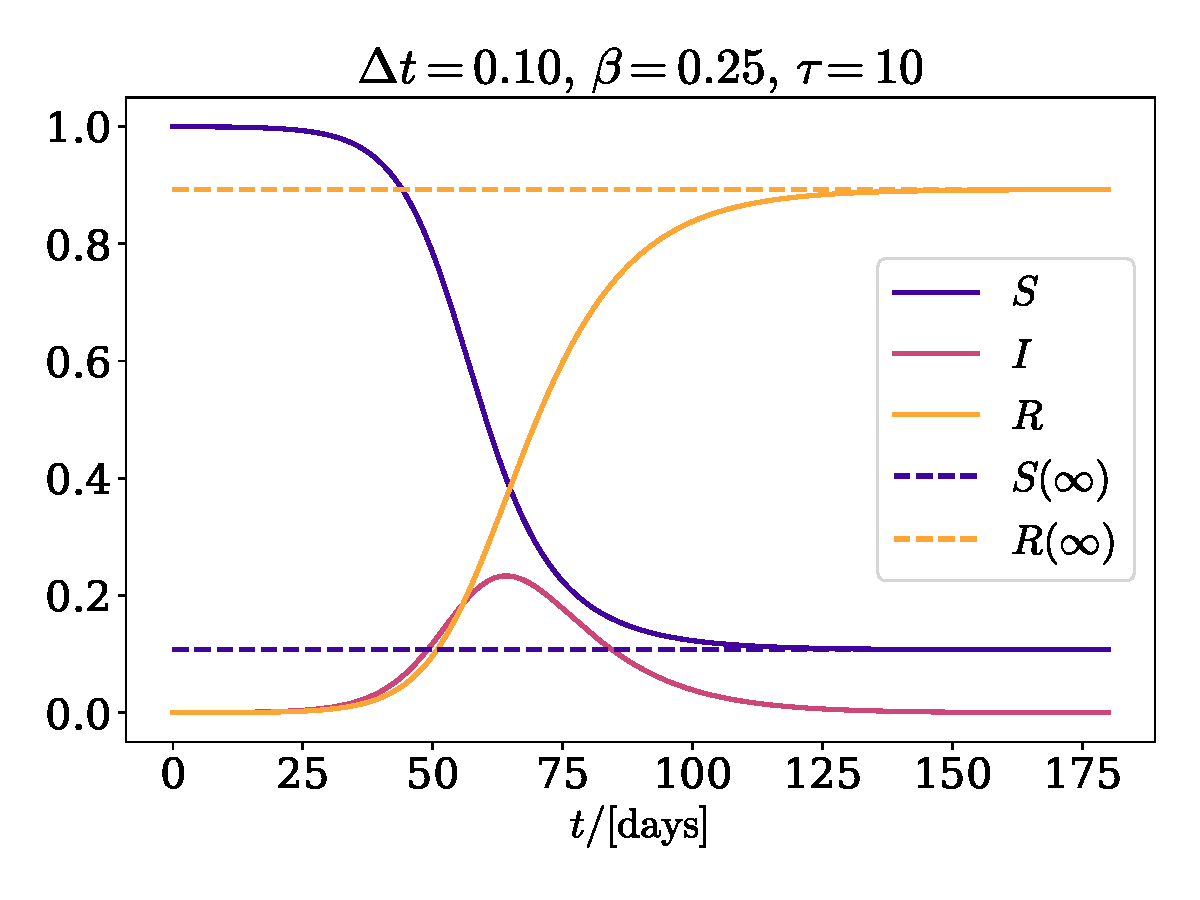
\includegraphics[width=.49\textwidth]{../plots/2A/TestSIR}
        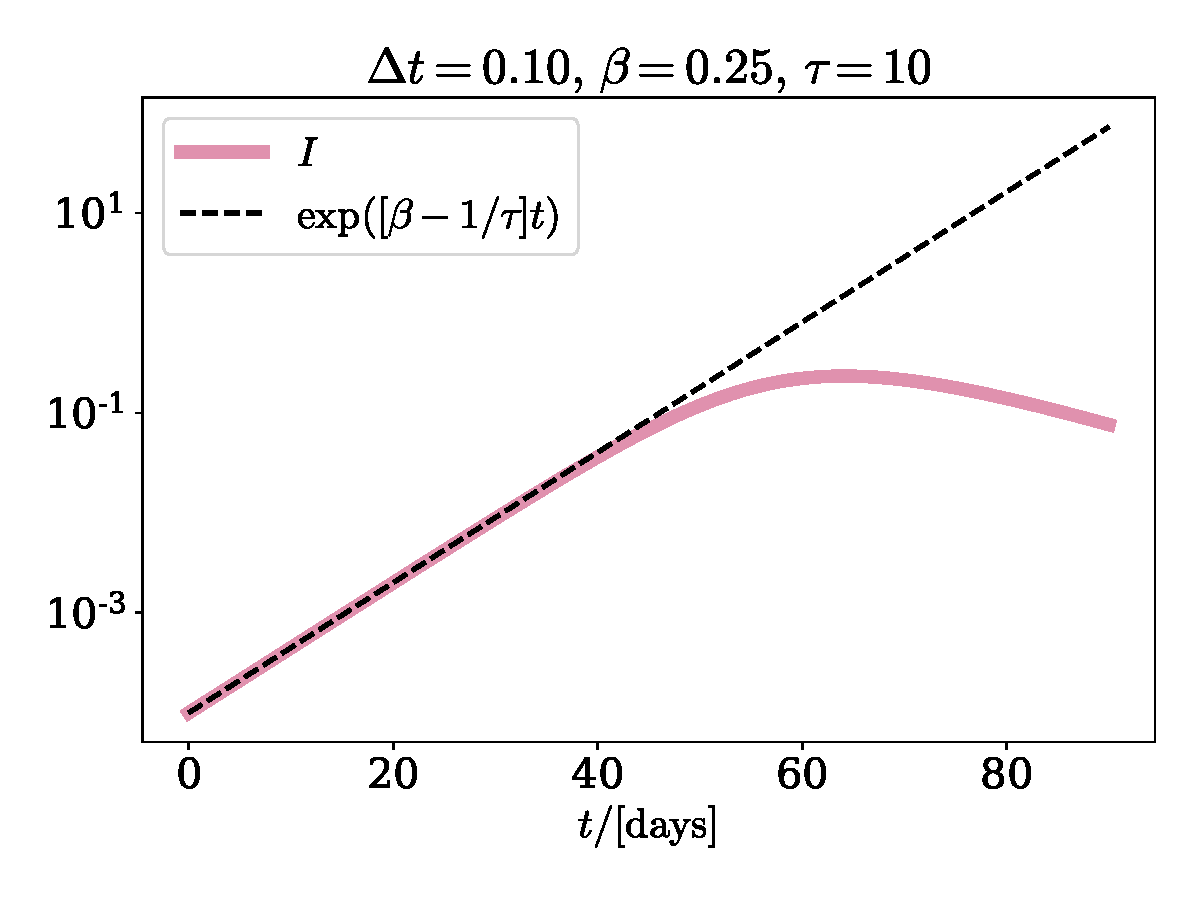
\includegraphics[width=.49\textwidth]{../plots/2A/TestI}
        \caption{On the left, the fraction of the population that is in each group, over time. The plot on the right shows how the infection spreads exponentially in the begining}
        \label{SIR}
    \end{figure}

    \begin{figure}[H]
        \centering
        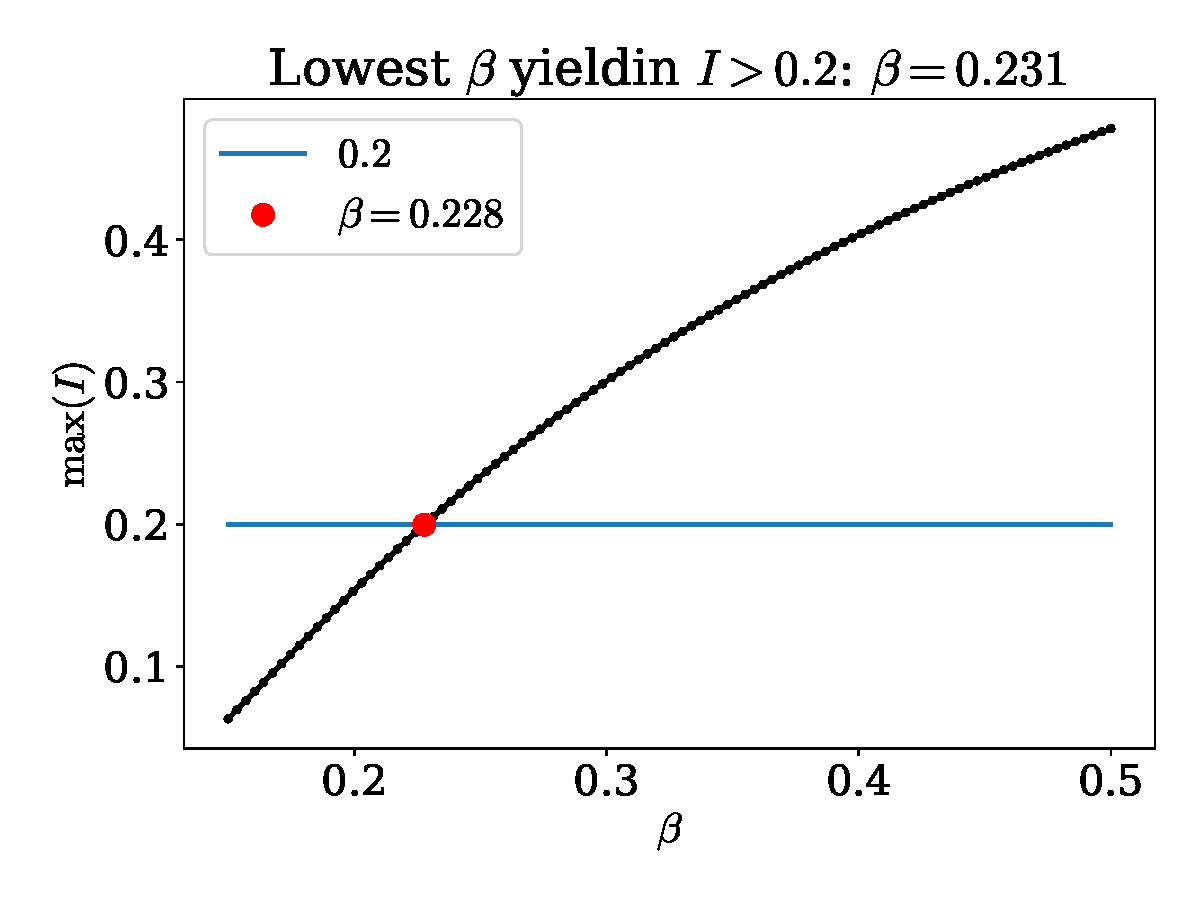
\includegraphics[width=.49\textwidth]{../plots/2A/flatten.pdf}
        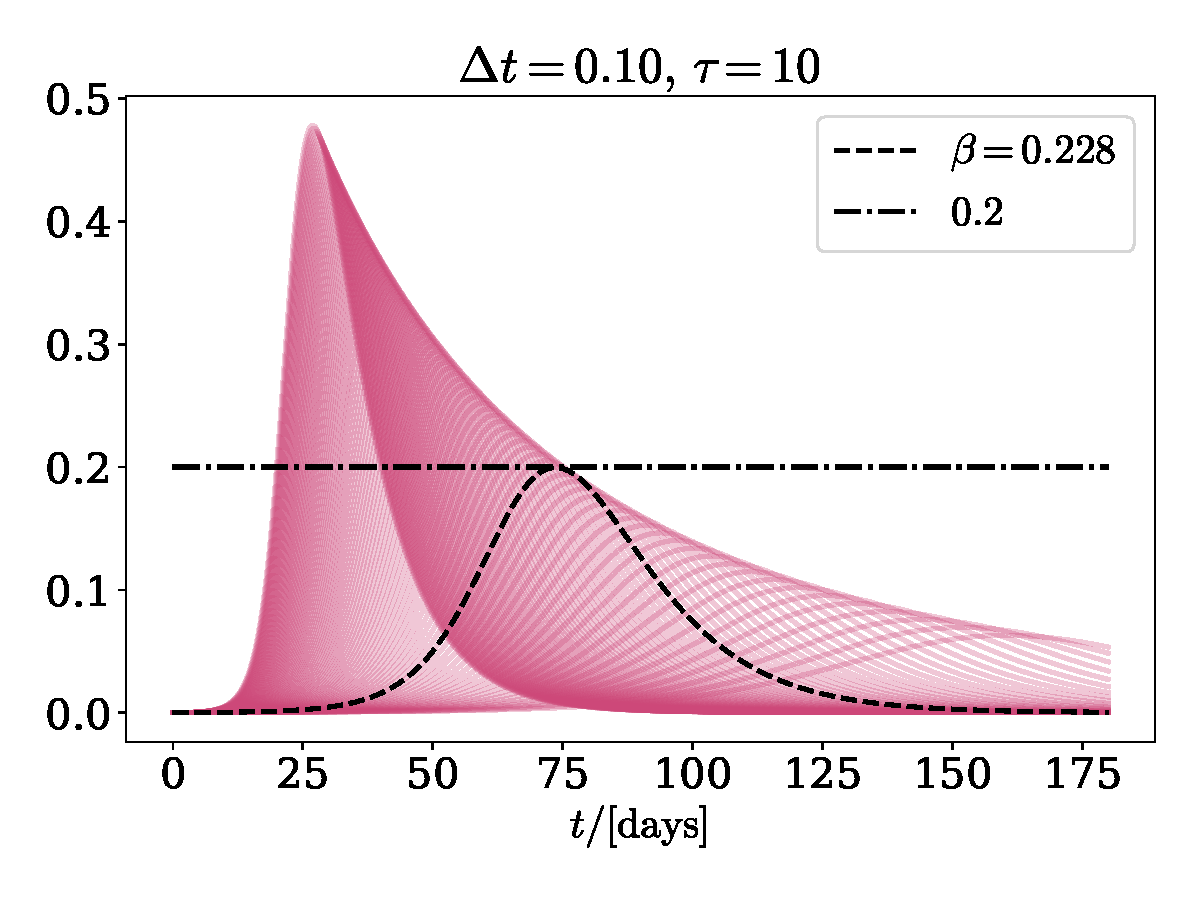
\includegraphics[width=.49\textwidth]{../plots/2A/flattenIs.pdf}
        \caption{The figure on th eright shows the maximum fraction of infected, as a function of $\beta$. The largest value of $\beta$ such that the maximum is beneth $0.2$ is indicated. On the right, the corresponding infection curves.}
        \label{flattening}
    \end{figure}

    \begin{figure}[H]
        \centering
        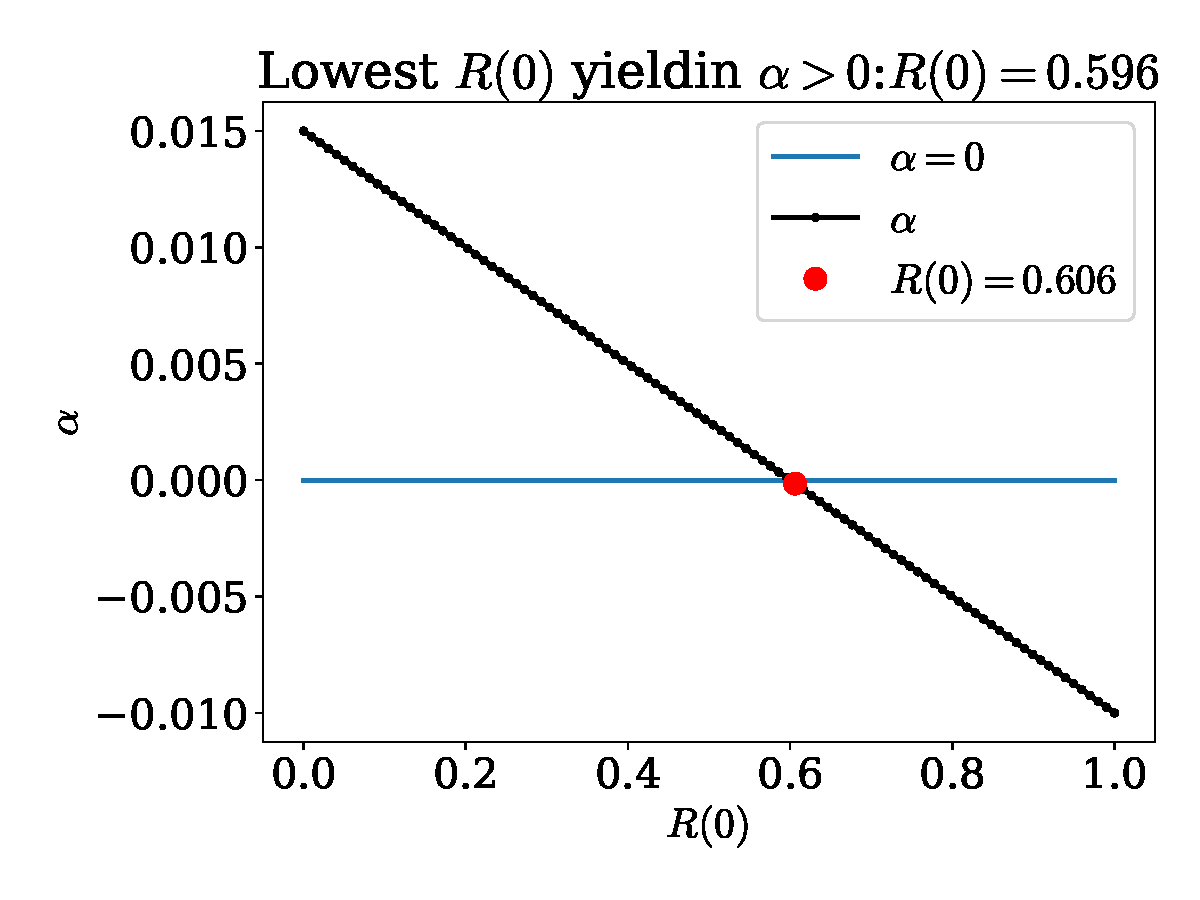
\includegraphics[width=.49\textwidth]{../plots/2A/vax.pdf}
        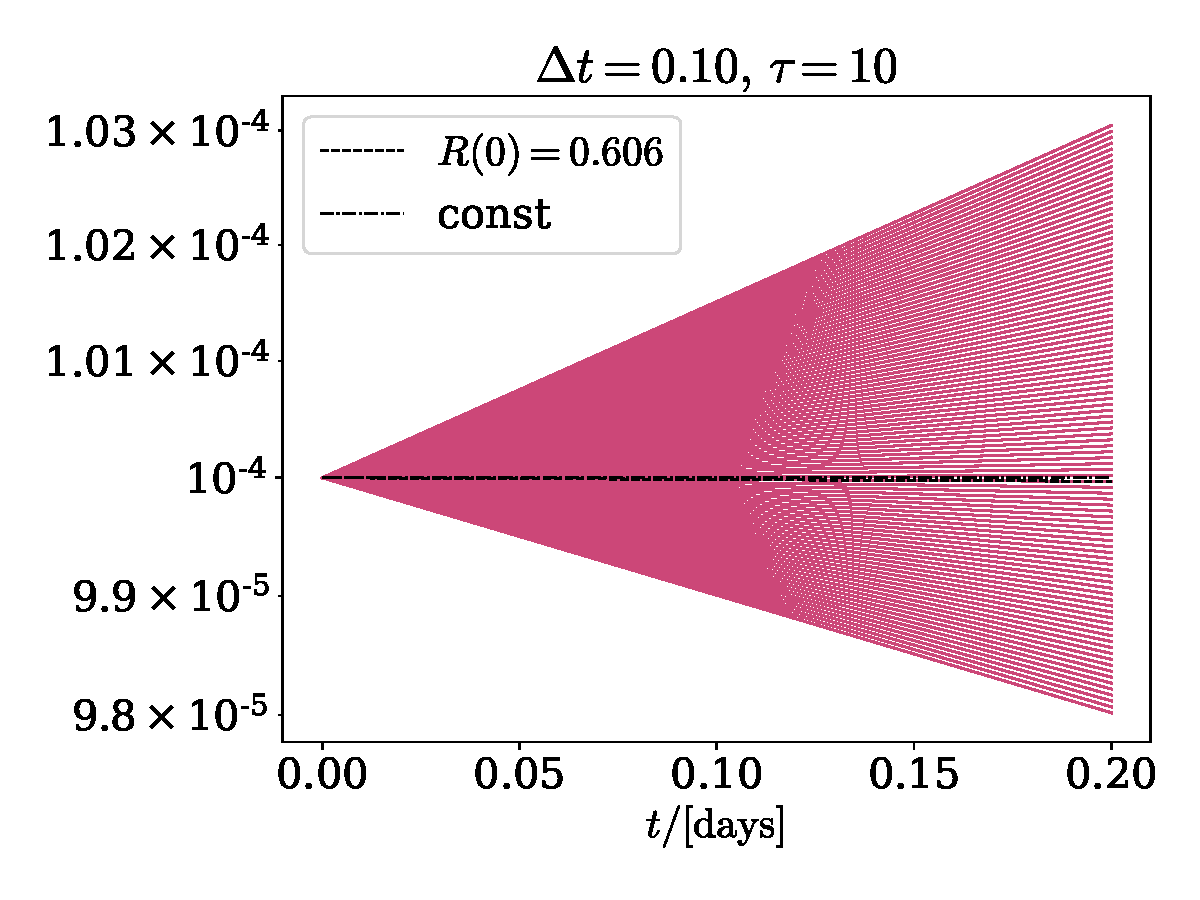
\includegraphics[width=.49\textwidth]{../plots/2A/vax_R.pdf}
        \caption{The plot on the left shows the maximu $R(0)$, i.e. fraction of vaccinated, that still gives exponential growth. The right shows a log-plot of the growht of infected at the very begining.}
        \label{vax}
    \end{figure}

    \subsection*{Stochastic SIR model}
    % TODO: Sjekke feil pga skrittlengde, differanse i siste punkt til analytisk løsning/asymptote s.f.a skrittlengde
    Next, the stochastic version of SIR model is used. \autoref{stochastic SIR} shows the result of 100 runs, which all give result close to that of the deterministic one. 
    All simulation uses a population of 100\,000, but the plots are normalized. 
    (DISCUSS TIMESTEP) 
    Due to the stochastic there is a difference in exactly when the spread takes of, but as the figure on the right show, when it does, it grows exponentially at the same rate as the deterministic model. 
    This is also the reason for the spread of the runs around the dashed line in the figure on the right.
    The early days of the infection is susceptible to fluctuations.
    We also see the stochastic model tend to be later than the deterministic.
    (THIS MIGHT HAVE SOMETHING TO DO WITH THE INITIAL CONDITIONS).
    The stochastic nature of this model makes it possible for the infection to die out, even with $\mathcal{R}_0>1$, by pure chance. 
    \autoref{Disappear} shows a probability for the infection terminating without spreading through the population, for different number of initially infected $I(0)$.
    This data is obtained by running the simulation 1\,000 for each initial condition, and terminating when it either reach $100$ infected, or $0$.
    $100$ infected is observed to yield very high probability of the disease spreading exponentially, and is thus used as a proxy for this.
    This assumption is backed up by the result shown in the figure, where the probability for the infection stopping early is negligible already at $I=10$.

    \begin{figure}[H]
        \centering
        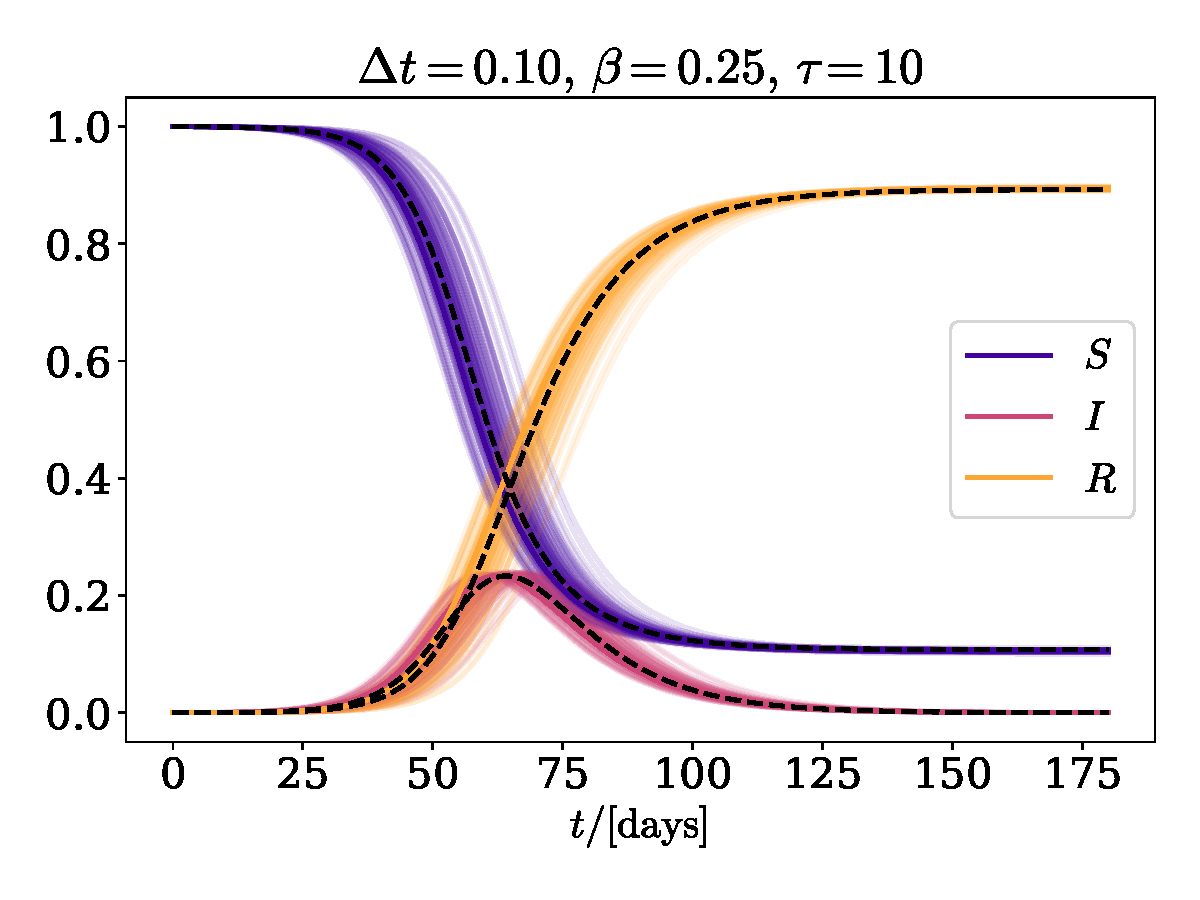
\includegraphics[width=.49\textwidth]{../plots/2B/TestSIR_stoch.pdf}
        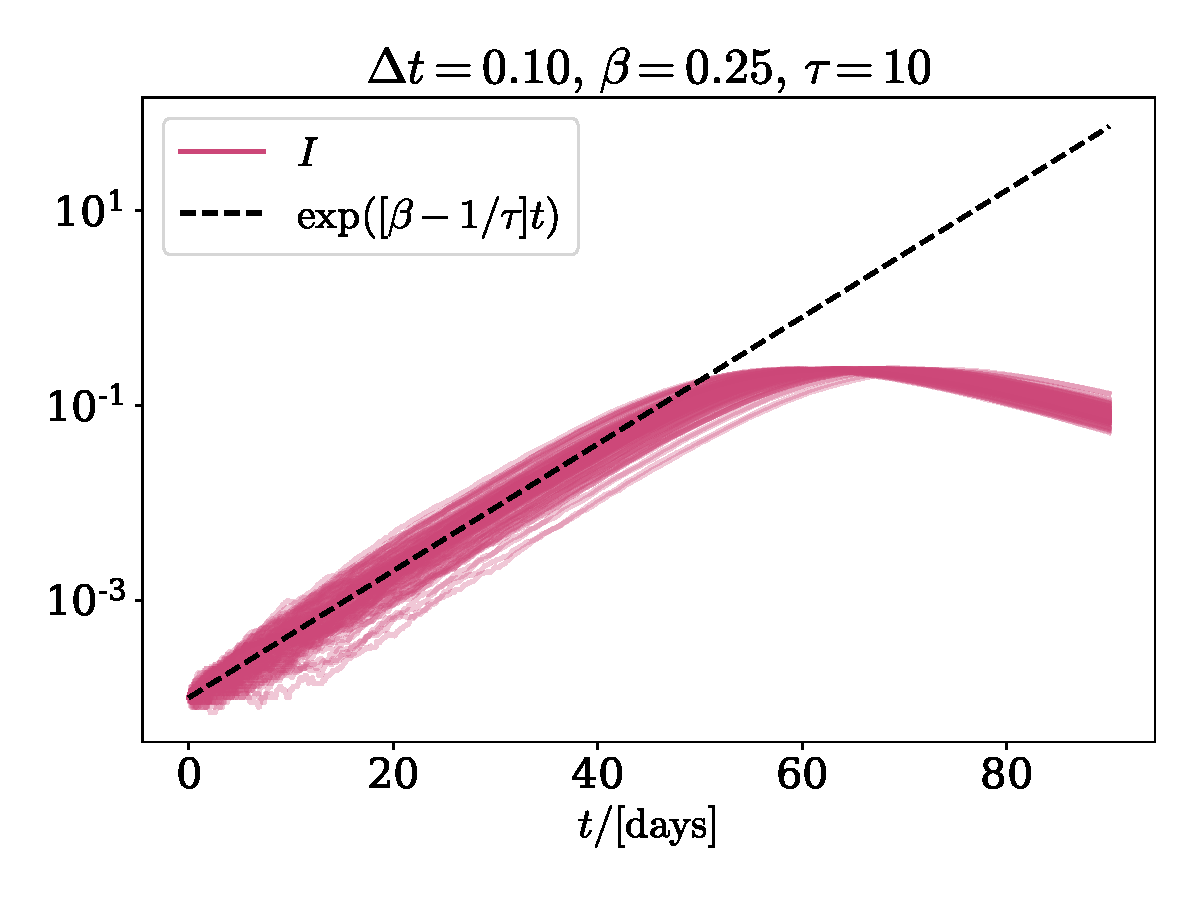
\includegraphics[width=.49\textwidth]{../plots/2B/TestI_stoch.pdf}
        \caption{100 runs of the stochastic SIR model. All runs are close to the deterministic, showed as dashed lines}
        \label{stochastic SIR}
    \end{figure}

    \begin{figure}[H]
        \centering
        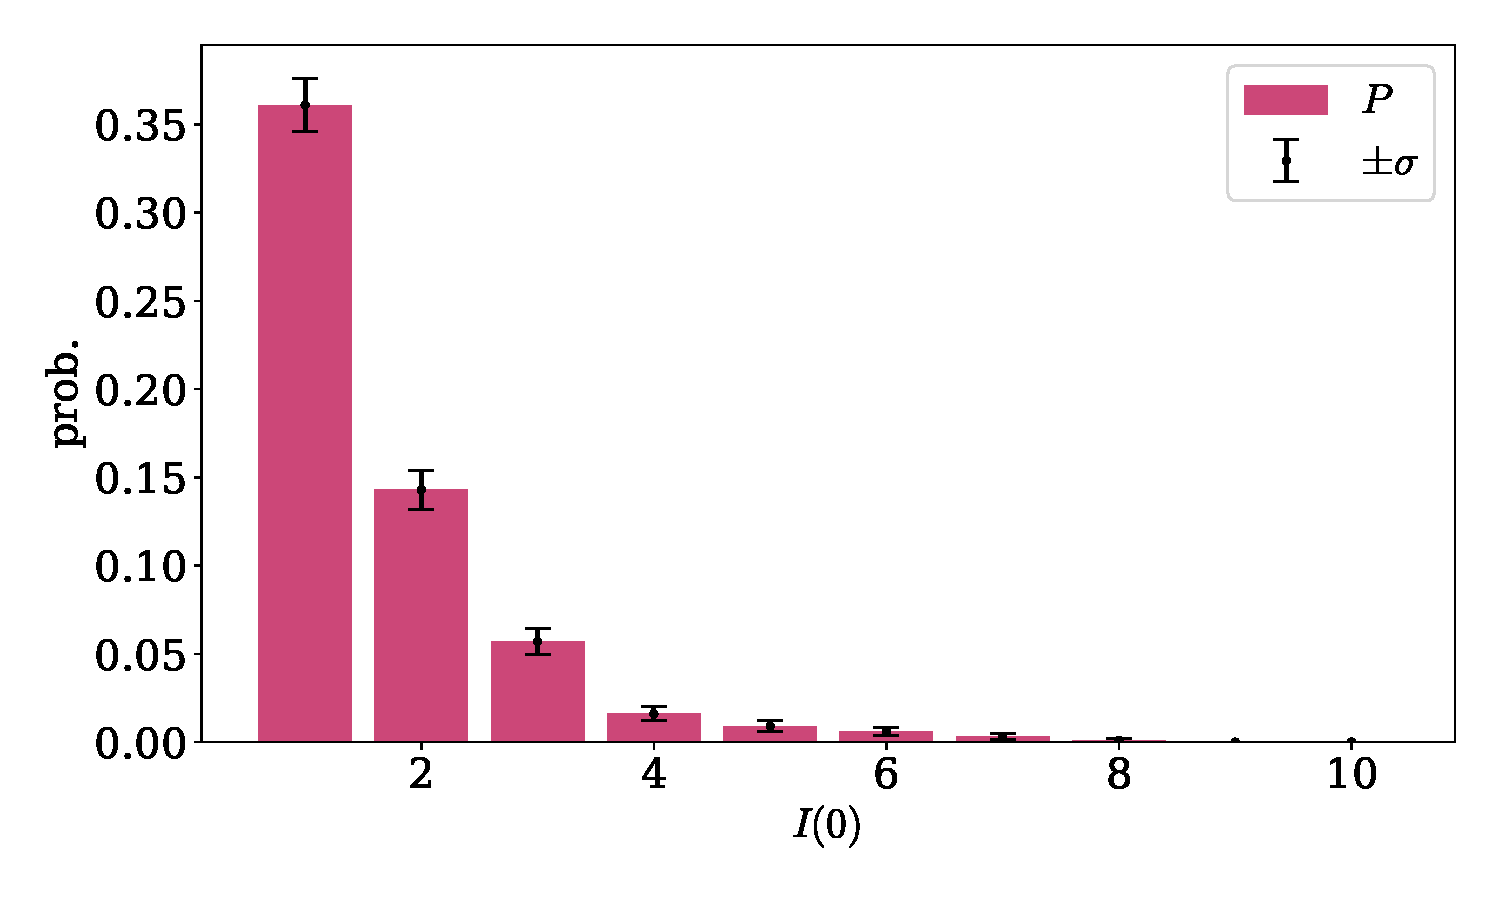
\includegraphics[width=.7\textwidth]{../plots/2B/disappear.pdf}
        \caption{The probability that the infection dies, for different starting values of $I$. Each probability is caculated from an average of 1\,000 runs.}
        \label{Disappear}
    \end{figure}

    \subsection*{SEIIaR model}
    The SEIIaR model incorporates the possibility of asymptomatic infection, $I_a$, as well as a incubation period, $E$, as well as a set of new parameters, described in \cite{exam}.
    \autoref{SEIIaR} shows 10 runs of the simulation, and compares it to the result from the deterministic SIR model.
    The same asymptotic values are reach for $S$ and $R$, however, due to the incubation period, the raise in infection is delayed somewhat.
    Infected people with symptoms, $I$, can self isolate, and thus decrease the spread of the disease.
    This is controlled by the $r_a$ parameter.
    If it is $1$, the symptomatic are as likely to infect others as $\mathcal{R}_0 = \beta \tau $ would suggest. 
    However, if it is less, for example due to isolation, then the spread will subside.
    \autoref{isolation} shows the early evolution of the exposed population, $E$, for $r_s\in [0, 1]$.
    Each line is an average of 100 runs.
    Due to this population not being infectious, it will initially decrease.
    The measure of the exponential increase is therefore taken as $\alpha = \ln\left(E(20)/E(5)\right)/(15 \mathrm{days})$.
    The largest $r_s$ that do not result in exponential growth is $r_s = 0.40$
    
    \begin{figure}[H]
        \centering
        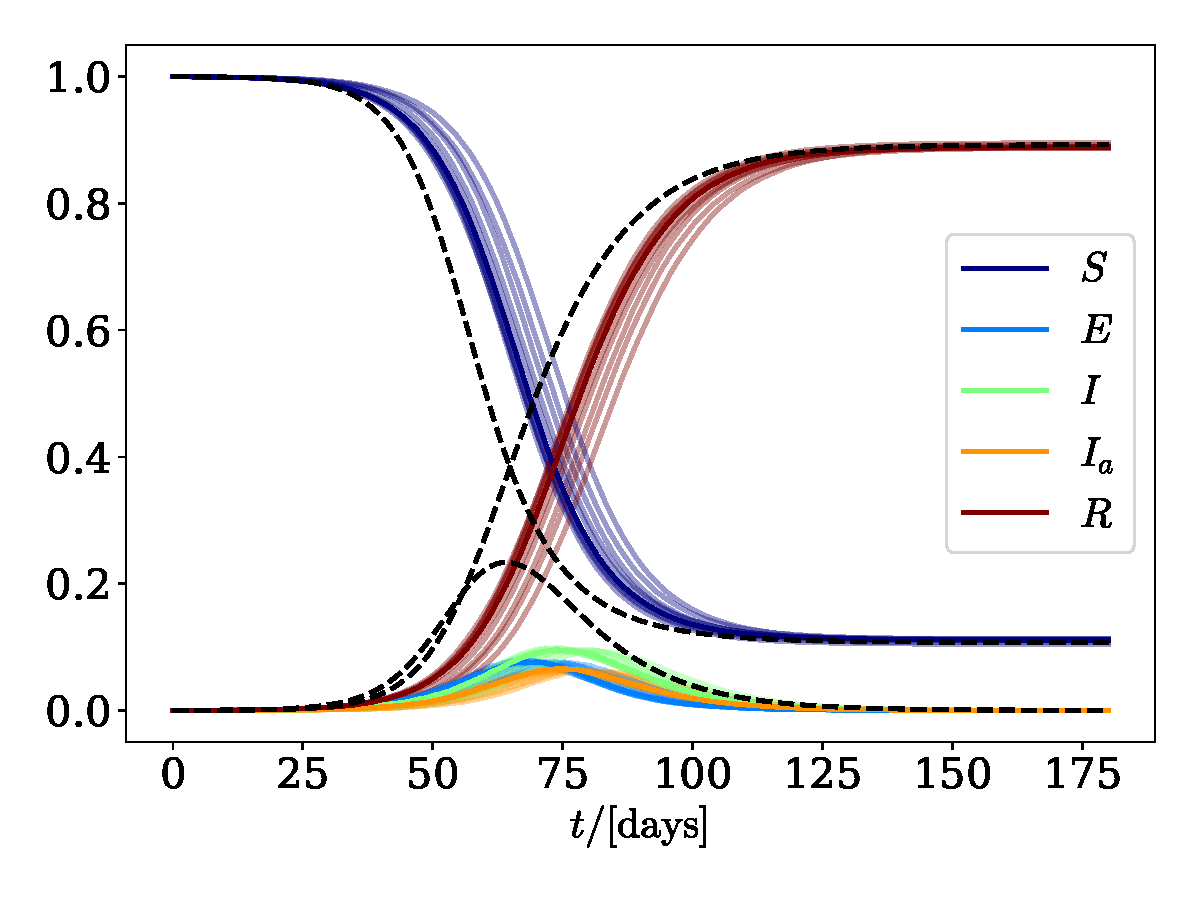
\includegraphics[width=.7\textwidth]{../plots/2C/TestSEIIaR.pdf}
        \caption{cap}
        \label{SEIIaR}
    \end{figure}

    \begin{figure}[H]
        \centering
        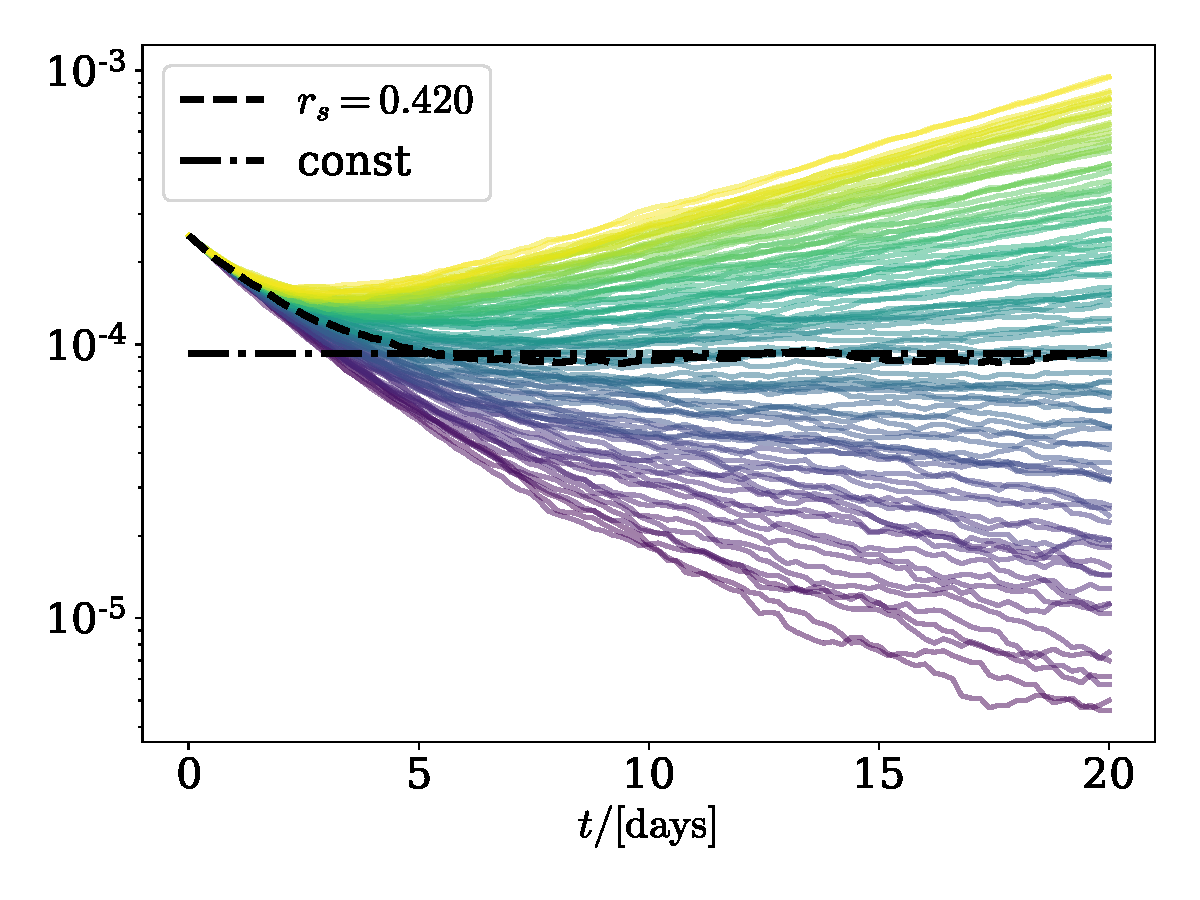
\includegraphics[width=.7\textwidth]{../plots/2C/isolation.pdf}
        \caption{cap}
        \label{isolation}
    \end{figure}


    \subsection*{SEIIaR commuter model}
    The last complication of the model is to include the fact that people live and work at different places, and might bring with them the infection when commuting. 
    The traveling pattern of the population is encoded in a matrix, as described in \cite{exam}.
    Given a matrix without off diagonal elements, each city should have evolve exactly as they do in the non-commuter SEIIaR test.
    This is thus a good check on the implementation.
    \autoref{test SEIIaR commute} shows the result in one of the cities of such a run in.
    This city did not have any commuters, and the same initial conditions, and should therefore yield identical results, modulo the inherit randomness of the, which a comparison with \autoref{SEIIaR} confirms.
    Next, the system described by the matrix in Equation 10 in \cite{exam} is simulated.
    The result in each town is showed in \autoref{two towns}
    (ADD MORE DATA: WHEN DO THEY PEAK; WHAT ARE THE ASYMPTOTES. DISCUSS)


    \begin{figure}[H]
        \centering
        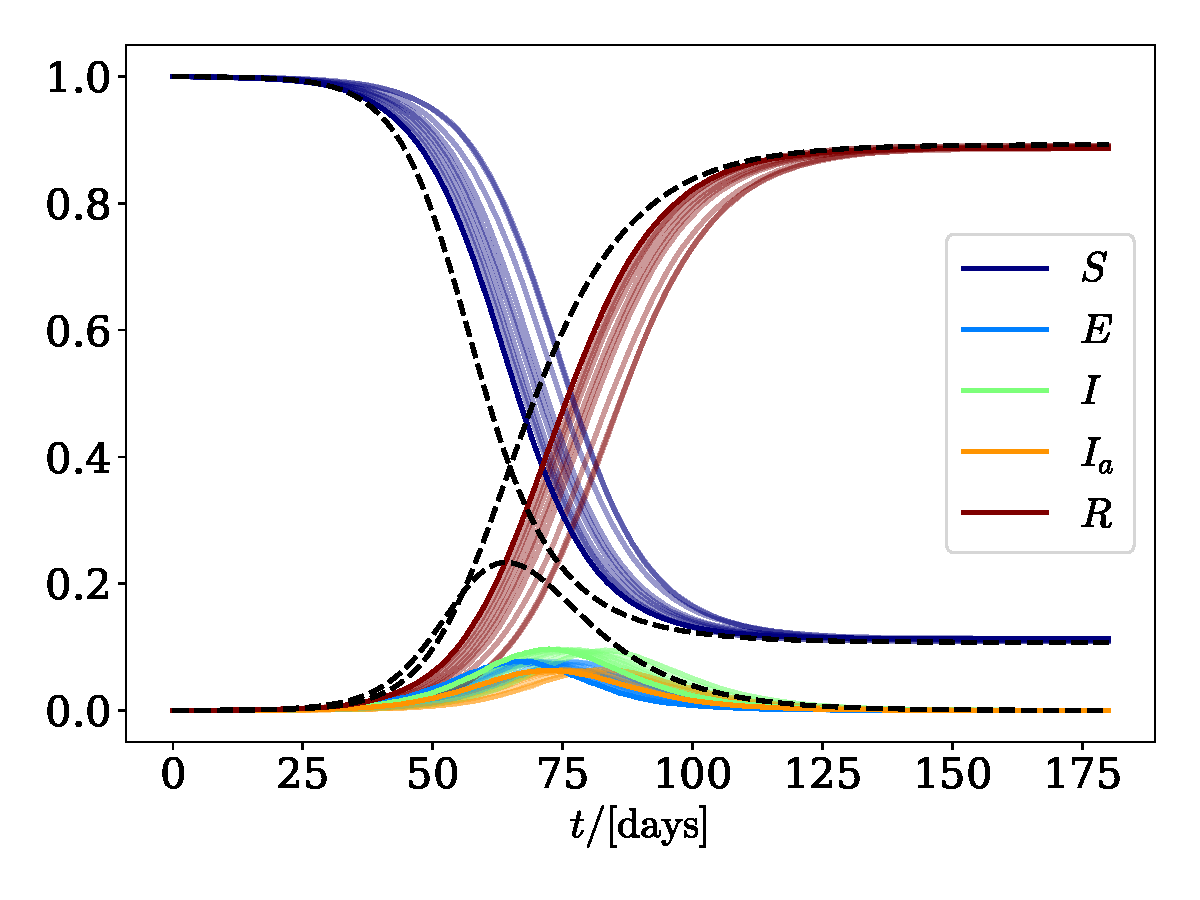
\includegraphics[width=.7\textwidth]{../plots/2D/TestSEIIaR_commute.pdf}
        \caption{cap}
        \label{test SEIIaR commute}
    \end{figure}

    \begin{figure}[H]
        \centering
        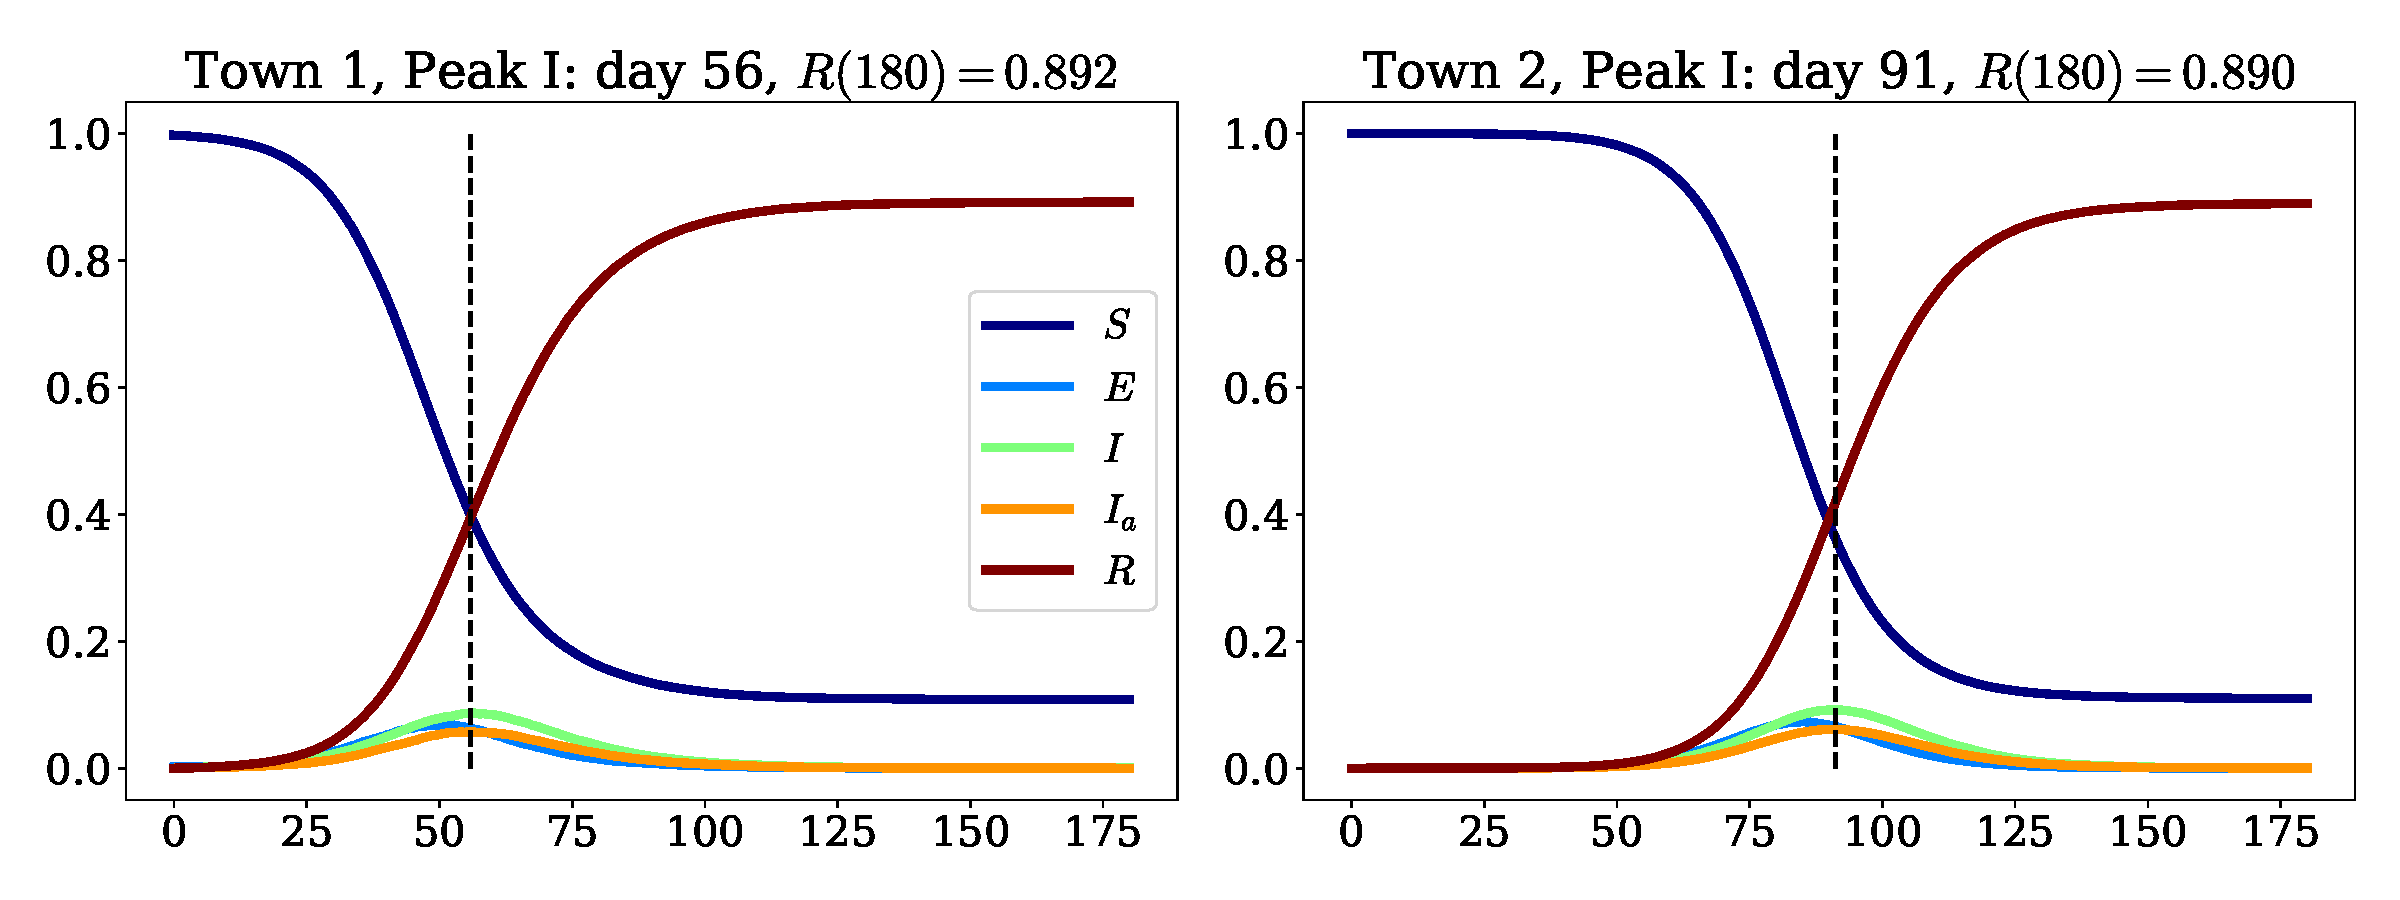
\includegraphics[width=.7\textwidth]{../plots/2D/two_towns.pdf}
        \caption{cap}
        \label{two towns}
    \end{figure}


    \printbibliography
\end{document}